\documentclass[]{article}
\usepackage{lmodern}
\usepackage{amssymb,amsmath}
\usepackage{ifxetex,ifluatex}
\usepackage{fixltx2e} % provides \textsubscript
\ifnum 0\ifxetex 1\fi\ifluatex 1\fi=0 % if pdftex
  \usepackage[T1]{fontenc}
  \usepackage[utf8]{inputenc}
\else % if luatex or xelatex
  \ifxetex
    \usepackage{mathspec}
    \usepackage{xltxtra,xunicode}
  \else
    \usepackage{fontspec}
  \fi
  \defaultfontfeatures{Mapping=tex-text,Scale=MatchLowercase}
  \newcommand{\euro}{€}
\fi
% use upquote if available, for straight quotes in verbatim environments
\IfFileExists{upquote.sty}{\usepackage{upquote}}{}
% use microtype if available
\IfFileExists{microtype.sty}{%
\usepackage{microtype}
\UseMicrotypeSet[protrusion]{basicmath} % disable protrusion for tt fonts
}{}
\ifxetex
  \usepackage[setpagesize=false, % page size defined by xetex
              unicode=false, % unicode breaks when used with xetex
              xetex]{hyperref}
\else
  \usepackage[unicode=true]{hyperref}
\fi
\hypersetup{breaklinks=true,
            bookmarks=true,
            pdfauthor={},
            pdftitle={},
            colorlinks=true,
            citecolor=blue,
            urlcolor=blue,
            linkcolor=magenta,
            pdfborder={0 0 0}}
\urlstyle{same}  % don't use monospace font for urls
\usepackage{color}
\usepackage{fancyvrb}
\newcommand{\VerbBar}{|}
\newcommand{\VERB}{\Verb[commandchars=\\\{\}]}
\DefineVerbatimEnvironment{Highlighting}{Verbatim}{commandchars=\\\{\}}
% Add ',fontsize=\small' for more characters per line
\newenvironment{Shaded}{}{}
\newcommand{\KeywordTok}[1]{\textcolor[rgb]{0.00,0.44,0.13}{\textbf{{#1}}}}
\newcommand{\DataTypeTok}[1]{\textcolor[rgb]{0.56,0.13,0.00}{{#1}}}
\newcommand{\DecValTok}[1]{\textcolor[rgb]{0.25,0.63,0.44}{{#1}}}
\newcommand{\BaseNTok}[1]{\textcolor[rgb]{0.25,0.63,0.44}{{#1}}}
\newcommand{\FloatTok}[1]{\textcolor[rgb]{0.25,0.63,0.44}{{#1}}}
\newcommand{\ConstantTok}[1]{\textcolor[rgb]{0.53,0.00,0.00}{{#1}}}
\newcommand{\CharTok}[1]{\textcolor[rgb]{0.25,0.44,0.63}{{#1}}}
\newcommand{\SpecialCharTok}[1]{\textcolor[rgb]{0.25,0.44,0.63}{{#1}}}
\newcommand{\StringTok}[1]{\textcolor[rgb]{0.25,0.44,0.63}{{#1}}}
\newcommand{\VerbatimStringTok}[1]{\textcolor[rgb]{0.25,0.44,0.63}{{#1}}}
\newcommand{\SpecialStringTok}[1]{\textcolor[rgb]{0.73,0.40,0.53}{{#1}}}
\newcommand{\ImportTok}[1]{{#1}}
\newcommand{\CommentTok}[1]{\textcolor[rgb]{0.38,0.63,0.69}{\textit{{#1}}}}
\newcommand{\DocumentationTok}[1]{\textcolor[rgb]{0.73,0.13,0.13}{\textit{{#1}}}}
\newcommand{\AnnotationTok}[1]{\textcolor[rgb]{0.38,0.63,0.69}{\textbf{\textit{{#1}}}}}
\newcommand{\CommentVarTok}[1]{\textcolor[rgb]{0.38,0.63,0.69}{\textbf{\textit{{#1}}}}}
\newcommand{\OtherTok}[1]{\textcolor[rgb]{0.00,0.44,0.13}{{#1}}}
\newcommand{\FunctionTok}[1]{\textcolor[rgb]{0.02,0.16,0.49}{{#1}}}
\newcommand{\VariableTok}[1]{\textcolor[rgb]{0.10,0.09,0.49}{{#1}}}
\newcommand{\ControlFlowTok}[1]{\textcolor[rgb]{0.00,0.44,0.13}{\textbf{{#1}}}}
\newcommand{\OperatorTok}[1]{\textcolor[rgb]{0.40,0.40,0.40}{{#1}}}
\newcommand{\BuiltInTok}[1]{{#1}}
\newcommand{\ExtensionTok}[1]{{#1}}
\newcommand{\PreprocessorTok}[1]{\textcolor[rgb]{0.74,0.48,0.00}{{#1}}}
\newcommand{\AttributeTok}[1]{\textcolor[rgb]{0.49,0.56,0.16}{{#1}}}
\newcommand{\RegionMarkerTok}[1]{{#1}}
\newcommand{\InformationTok}[1]{\textcolor[rgb]{0.38,0.63,0.69}{\textbf{\textit{{#1}}}}}
\newcommand{\WarningTok}[1]{\textcolor[rgb]{0.38,0.63,0.69}{\textbf{\textit{{#1}}}}}
\newcommand{\AlertTok}[1]{\textcolor[rgb]{1.00,0.00,0.00}{\textbf{{#1}}}}
\newcommand{\ErrorTok}[1]{\textcolor[rgb]{1.00,0.00,0.00}{\textbf{{#1}}}}
\newcommand{\NormalTok}[1]{{#1}}
\usepackage{graphicx,grffile}
\makeatletter
\def\maxwidth{\ifdim\Gin@nat@width>\linewidth\linewidth\else\Gin@nat@width\fi}
\def\maxheight{\ifdim\Gin@nat@height>\textheight\textheight\else\Gin@nat@height\fi}
\makeatother
% Scale images if necessary, so that they will not overflow the page
% margins by default, and it is still possible to overwrite the defaults
% using explicit options in \includegraphics[width, height, ...]{}
\setkeys{Gin}{width=\maxwidth,height=\maxheight,keepaspectratio}
\setlength{\parindent}{0pt}
\setlength{\parskip}{6pt plus 2pt minus 1pt}
\setlength{\emergencystretch}{3em}  % prevent overfull lines
\providecommand{\tightlist}{%
  \setlength{\itemsep}{0pt}\setlength{\parskip}{0pt}}
\setcounter{secnumdepth}{0}

\date{}

% Redefines (sub)paragraphs to behave more like sections
\ifx\paragraph\undefined\else
\let\oldparagraph\paragraph
\renewcommand{\paragraph}[1]{\oldparagraph{#1}\mbox{}}
\fi
\ifx\subparagraph\undefined\else
\let\oldsubparagraph\subparagraph
\renewcommand{\subparagraph}[1]{\oldsubparagraph{#1}\mbox{}}
\fi

\begin{document}
	\title{\huge\textbf{Pose Estimation}\LARGE \\Project: Marker-based Localization}
	\author{Niharika Jayanthi, Dheeraj Kamath \\Mentor: Sanam Shakya}
	\maketitle
	\pagebreak
\section{Goals}\label{goals}

\begin{itemize}
\tightlist
\item
  To determine the pose of the camera
\item
  Using \textbf{cv2.solvePnP()}, \textbf{cv2.solvePnPRansac()} and
  \textbf{cv2.Rodrigues()} functions
\end{itemize}

\section{Prerequisites}\label{prerequisites}

\begin{itemize}
\tightlist
\item
  \href{https://github.com/eyantrainternship/eYSIP_2015_Marker_based_Robot_Localisation/wiki/Camera-Calibration}{Camera
  calibration}
\end{itemize}

\section{Theory}\label{theory}

Pose of an object refers to its position and orientation with respect to
the camera. To determine the pose, we need to solve the
perspective-n-point problem. In perspective-n-point problem, we are
given a set of object points and their corresponding image points and we
should determine the pose of the image. Trigonometric operations are
applied to find the solution. Refer to resources to learn in detail.

The pose of an object is represented in the form of its rotational
vector and translational vector. We have seen in camera calibration that
using cv2.calibrateCamera() function, we already obtain these two
vectors. So why do we need an alternative method to get this
information? cv2.calibrateCamera() has a lot of processing, so it
consumes more time. Instead, we save the camera matrix and distortion
coefficients obtained from cv2.calibrateCamera() and use them in
cv2.solvePnP() or cv2.solvePnPRansac() functions.

cv2.solvePnPRansac is better than cv2.solvePnP because this function
finds such a pose that minimizes reprojection error, that is, the sum of
squared distances between the observed projections imagePoints and the
projected objectPoints. The use of RANSAC makes the function resistant
to outliers.

Now, after finding the translational vector (tvec) and rotational vector
(rvec), we need to extract the required information from them. The
distance from camera is acquired from the Z-coordinate in the tvec. This
is because we assume the object is always on Z=0 plane and the camera is
put at a distance from it. The x-coordinate in tvec denotes the
displacement between the origin object and camera axis in x-direction.
The angle is obtained from rvec. But first, we need to convert it into a
rotation matrix(R). This is done using cv2.Rodrigues() function. After
obtaining the matrix, we compare it to the rotational matrix of y-axis.

\begin{figure}[htbp]
\centering
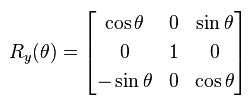
\includegraphics{images/Pose Estimation/Rotation matrix.JPG}
\caption{Rotation matrix in y-axis}
\end{figure}
\pagebreak
We then take the sine inverse of R{[}0{]}{[}2{]}. This gives us the
angle of inclination. The following image depicts this-

\begin{figure}[htbp]
\centering
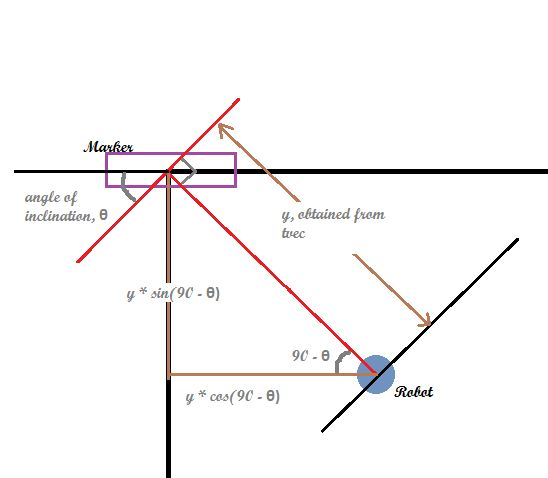
\includegraphics[width = 11cm]{images/Pose Estimation/Pose.JPG}
\caption{Pose estimation}
\end{figure}
\pagebreak
\section{Code}\label{code}

The main functions and their parameters are-

\emph{\textbf{cv2.solvePnP(objectPoints, imagePoints, cameraMatrix,
distCoeffs{[}, rvec{[}, tvec{[}, useExtrinsicGuess{[},
flags{]}{]}{]}{]}) → retval, rvec, tvec}}

where

\begin{itemize}
\item
  \textbf{objectPoints} -- Array of object points in the object
  coordinate space, 3xN/Nx3 1-channel or 1xN/Nx1 3-channel, where N is
  the number of points.
\item
  \textbf{imagePoints} -- Array of corresponding image points, 2xN/Nx2
  1-channel or 1xN/Nx1 2-channel, where N is the number of points.
\item
  \textbf{cameraMatrix} -- Input camera matrix
\item
  \textbf{distCoeffs} -- Input vector of distortion coefficients (k\_1,
  k\_2, p\_1, p\_2{[}, k\_3{[}, k\_4, k\_5, k\_6{]}{]}) of 4, 5, or 8
  elements. If the vector is NULL/empty, the zero distortion
  coefficients are assumed.
\item
  \textbf{rvec} -- Output rotation vector (see Rodrigues() ) that,
  together with tvec , brings points from the model coordinate system to
  the camera coordinate system.
\item
  \textbf{tvec} -- Output translation vector
\item
  \textbf{useExtrinsicGuess} -- If true (1), the function uses the
  provided rvec and tvec values as initial approximations of the
  rotation and translation vectors, respectively, and further optimizes
  them.
\item
  \textbf{flags} -- Method for solving a PnP problem:
\end{itemize}

\textbf{CV\_ITERATIVE Iterative}

\textbf{CV\_P3P}

\textbf{CV\_EPNP}

\begin{center}\rule{0.5\linewidth}{\linethickness}\end{center}

\emph{\textbf{cv2.solvePnPRansac(objectPoints, imagePoints,
cameraMatrix, distCoeffs{[}, rvec{[}, tvec{[}, useExtrinsicGuess{[},
iterationsCount{[}, reprojectionError{[}, minInliersCount{[},
inliers{[}, flags{]}{]}{]}{]}{]}{]}{]}{]}) → rvec, tvec, inliers}}

where -

\begin{itemize}
\item
  \textbf{objectPoints} -- Array of object points in the object
  coordinate space, 3xN/Nx3 1-channel or 1xN/Nx1 3-channel, where N is
  the number of points. vector can be also passed here.
\item
  \textbf{imagePoints} -- Array of corresponding image points, 2xN/Nx2
  1-channel or 1xN/Nx1 2-channel, where N is the number of points.
  vector can be also passed here.
\item
  \textbf{cameraMatrix} -- Input camera matrix
\item
  \textbf{distCoeffs} -- Input vector of distortion coefficients (k\_1,
  k\_2, p\_1, p\_2{[}, k\_3{[}, k\_4, k\_5, k\_6{]}{]}) of 4, 5, or 8
  elements. If the vector is NULL/empty, the zero distortion
  coefficients are assumed.
\item
  \textbf{rvec} -- Output rotation vector (see Rodrigues() ) that,
  together with tvec , brings points from the model coordinate system to
  the camera coordinate system.
\item
  \textbf{tvec} -- Output translation vector.
\item
  \textbf{useExtrinsicGuess} -- If true (1), the function uses the
  provided rvec and tvec values as initial approximations of the
  rotation and translation vectors, respectively, and further optimizes
  them.
\item
  \textbf{iterationsCount} -- Number of iterations. reprojectionError --
  Inlier threshold value used by the RANSAC procedure. The parameter
  value is the maximum allowed distance between the observed and
  computed point projections to consider it an inlier.
\item
  \textbf{minInliersCount} -- Number of inliers. If the algorithm at
  some stage finds more inliers than minInliersCount , it finishes.
\item
  \textbf{inliers} -- Output vector that contains indices of inliers in
  objectPoints and imagePoints .
\item
  \textbf{flags} -- Method for solving a PnP problem
\end{itemize}

\begin{center}\rule{0.5\linewidth}{\linethickness}\end{center}

\emph{\textbf{cv2.Rodrigues(src{[}, dst{[}, jacobian{]}{]}) → dst,
jacobian}}

where -

\begin{itemize}
\item
  \textbf{src} -- Input rotation vector (3x1 or 1x3) or rotation matrix
  (3x3).
\item
  \textbf{dst} -- Output rotation matrix (3x3) or rotation vector (3x1
  or 1x3), respectively.
\item
  \textbf{jacobian} -- Optional output Jacobian matrix, 3x9 or 9x3,
  which is a matrix of partial derivatives of the output array
  components with respect to the input array components.
\end{itemize}

The following code snippet depicts how to find pose-

\begin{Shaded}
\begin{Highlighting}[]
\NormalTok{mtx }\OperatorTok{=} \NormalTok{np.load(}\StringTok{'matrix.npy'}\NormalTok{)}
\NormalTok{dist }\OperatorTok{=} \NormalTok{np.load(}\StringTok{'distortion.npy'}\NormalTok{)}

\NormalTok{rvec, tvec, inliers }\OperatorTok{=} \NormalTok{cv2.solvePnPRansac(objp, imgp, mtx, dist)}
\BuiltInTok{print} \StringTok{"Rvec}\CharTok{\textbackslash{}n}\StringTok{"}\NormalTok{, rvec}
\BuiltInTok{print} \StringTok{"}\CharTok{\textbackslash{}n}\StringTok{Tvec"}\NormalTok{, tvec}


\NormalTok{dst, jacobian }\OperatorTok{=} \NormalTok{cv2.Rodrigues(rvec)}
\NormalTok{x }\OperatorTok{=} \NormalTok{tvec[}\DecValTok{0}\NormalTok{][}\DecValTok{0}\NormalTok{]}
\NormalTok{y }\OperatorTok{=} \NormalTok{tvec[}\DecValTok{2}\NormalTok{][}\DecValTok{0}\NormalTok{]}
\NormalTok{t }\OperatorTok{=} \NormalTok{(math.asin(}\OperatorTok{-}\NormalTok{dst[}\DecValTok{0}\NormalTok{][}\DecValTok{2}\NormalTok{]))}

\BuiltInTok{print} \StringTok{"X"}\NormalTok{, x, }\StringTok{"Y"}\NormalTok{, y, }\StringTok{"Angle"}\NormalTok{, t}
\BuiltInTok{print} \StringTok{"90-t"}\NormalTok{, (math.pi}\OperatorTok{/}\DecValTok{2}\NormalTok{) }\OperatorTok{-} \NormalTok{t}

\NormalTok{Rx }\OperatorTok{=} \NormalTok{y }\OperatorTok{*} \NormalTok{(math.cos((math.pi}\OperatorTok{/}\DecValTok{2}\NormalTok{) }\OperatorTok{-} \NormalTok{t))}
\NormalTok{Ry }\OperatorTok{=} \NormalTok{y }\OperatorTok{*} \NormalTok{(math.sin((math.pi}\OperatorTok{/}\DecValTok{2}\NormalTok{) }\OperatorTok{-} \NormalTok{t))}

\BuiltInTok{print} \StringTok{"rx"}\NormalTok{, Rx, }\StringTok{"ry"}\NormalTok{, Ry}
\end{Highlighting}
\end{Shaded}

\section{Resources}\label{resources}

\begin{itemize}
\tightlist
\item
  http://docs.opencv.org/modules/calib3d/doc/camera\_calibration\_and\_3d\_reconstruction.html
\item
  http://projekter.aau.dk/projekter/files/14427578/A\_Comparison\_of\_2D-3D\_Pose\_Estimation\_Methods.pdf
\item
  http://homepages.inf.ed.ac.uk/rbf/CVonline/LOCAL\_COPIES/MARBLE/high/pia/solving.htm
\end{itemize}

\end{document}
